\documentclass[11pt]{amsbook}

\usepackage{amsmath}
\usepackage{graphicx}
\graphicspath{ {images/} }
\usepackage[turkish]{babel}

%\usepackage{../HBSuerDemir}	% ------------------------
\usepackage{../Ceyhun}	% ------------------------
\usepackage{../amsTurkish}


\begin{document}
% ++++++++++++++++++++++++++++++++++++++
\hPage{032}
% ++++++++++++++++++++++++++++++++++++++

\begin{itemize}
\item[$\mathbf{Tanım}$ 1.5.2  $\quad$]  $\alpha$($d_i$) = $\underset{(j)}{enb\textrm{\textit{\"{u}}}y\textrm{\textit{\"{u}}}k}$ u($d_i$,$d_j$) olarak gösterilen, $d_i$ düğümüne ilişkin uzaklığın alabileceği enbüyük değere, $d_i$ düğümünün $\mathit{\underline{\textit{açıklığı}}}$ denir. \par
\end{itemize}

\begin{itemize}
\item[$\mathbf{Tanım}$ 1.5.3  $\quad$]  $\sigma$ = $\underset{i}{\textit{enküçük}}$ {$\alpha$($d_i$)} olarak tanımlanan, çizgideki enküçük düğüm açıklığına, çizgenin $\mathit{\underline{\textit{yarıçapı}}}$ $\sigma$ denir.\par

\item[Genellikle] bir çizgide açıklığı çizgenin yarıçapına eşit birden çok düğüm vardır.\par

\end{itemize}



\begin{itemize}
\item[$\mathbf{Tanım}$ 1.5.4  $\quad$]  Ö ile gösterilen ve açıklıkları yarıçapa eşit olan düğümlerin irgittiği altçizgiye, çizgenin $\mathit{\underline{\textit{özeği}}}$, özeği oluşturan düğümlere $\mathit{\underline{\textit{özek düğümleri}}}$ denir.\par
\end{itemize}

\begin{itemize}
\item[$\mathbf{Tanım}$ 1.5.5  $\quad$] Özek düğümlerinden aşlayan $\sigma$ uzunluktaki yollara $\mathit{\underline{\textit{yarıçapsal yol}}}$ denir.\par
\end{itemize}

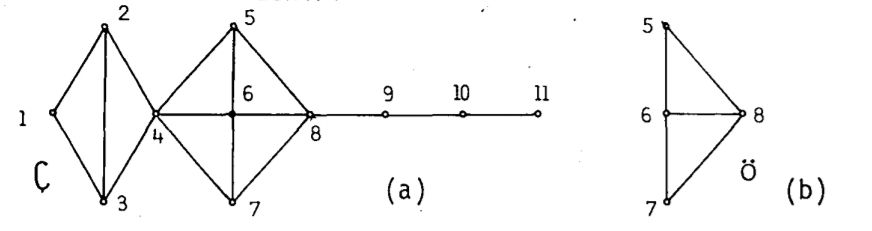
\includegraphics[width=500px]{images/sekil}
şekil 1.5.1 Açıklık, yarıçap ve özek

\end{document}